\documentclass[oneside,10pt]{book}

\usepackage{cdtBook}
\usepackage{usecases}

\title{SCVME}
\subtitle{Sistema de Compra y Venta de Material Electrónico}
\author{Sworkware}
%\organization{Escuela Superior de Cómputo, IPN}


%%%%%%%%%%%%%%%%%%%%%%%%%%%%%%%%%%%%%%%%%%%%%%%%%%%%%%%%%%%%%%%%
\begin{document}

\maketitle
\thispagestyle{empty}

\frontmatter
\tableofcontents

\mainmatter

%=========================================================
\chapter{Introducción}

\cfinput{introduccion}

%=========================================================
\chapter{Análisis del problema}

\cfinput{problematica}

%=========================================================
\chapter{Propuesta de solución}

\cfinput{propuesta}



%=========================================================
\chapter{Modelo de Negocios}

\cfinput{brGlosario}
\cfinput{brProceso}
\cfinput{brModelo}
\cfinput{brReglas}

%=========================================================
\chapter{Modelo del despliegue del sistema}

%=========================================================
\chapter{Modelo de comportamiento}
	
	\begin{figure}[htbp!]
		\centering
			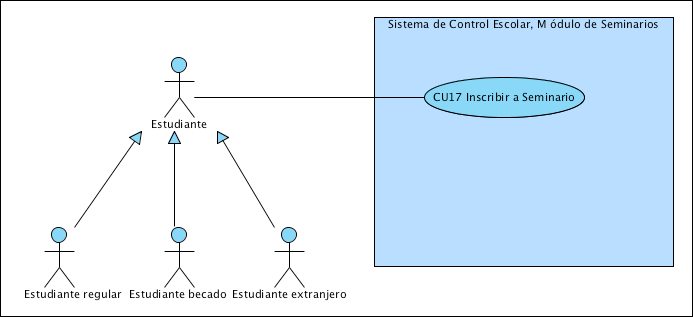
\includegraphics[width=0.8\textwidth]{images/CasosDeUso}
		\caption{Diagrama de Casos de Uso del sistema.}
	\end{figure}
	
	\begin{figure}[htbp!]
		\centering
			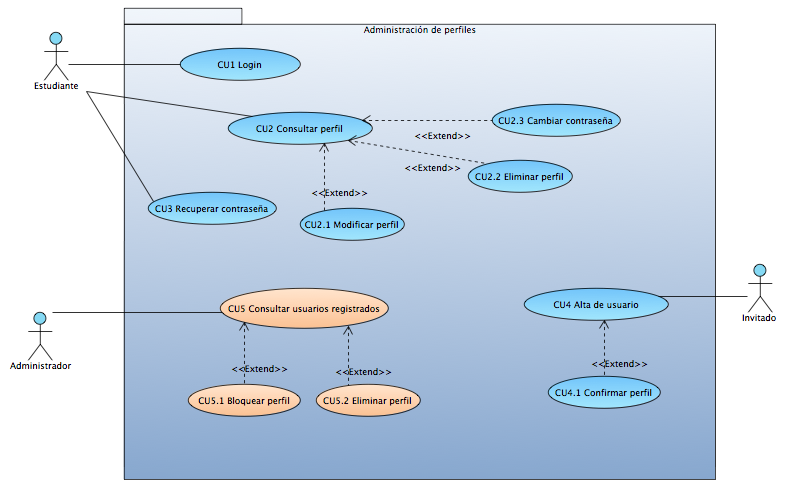
\includegraphics[width=0.8\textwidth]{images/CasosDeUso1}
		\caption{Diagrama de Casos de Uso del sistema.}
	\end{figure}
	
	\begin{figure}[htbp!]
		\centering
			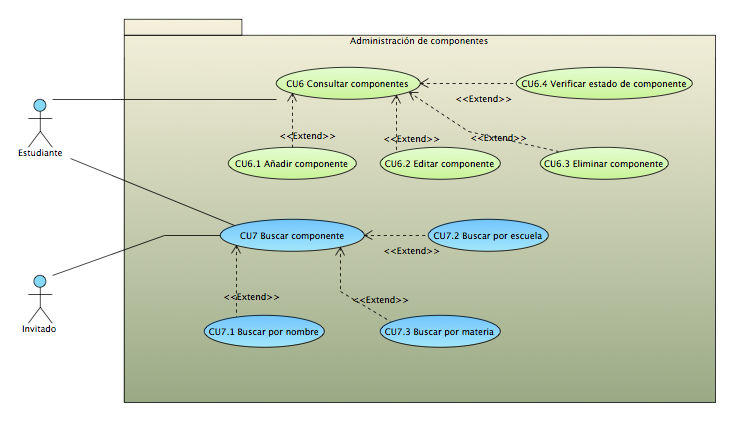
\includegraphics[width=0.8\textwidth]{images/CasosDeUso2}
		\caption{Diagrama de Casos de Uso del sistema.}
	\end{figure}
	
	\begin{figure}[htbp!]
		\centering
			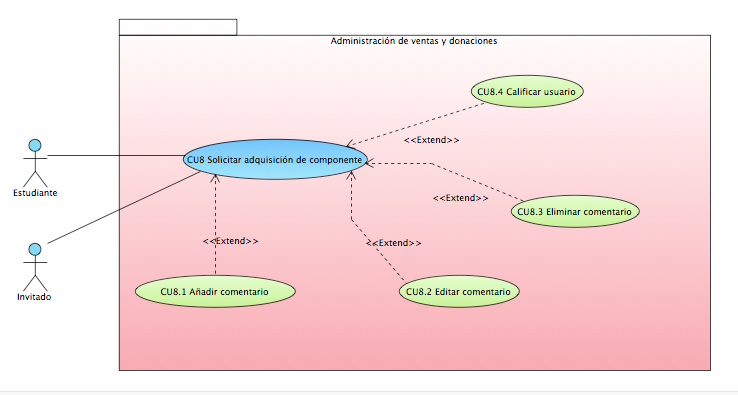
\includegraphics[width=0.8\textwidth]{images/CasosDeUso3}
		\caption{Diagrama de Casos de Uso del sistema.}
	\end{figure}
	
	\begin{figure}[htbp!]
		\centering
			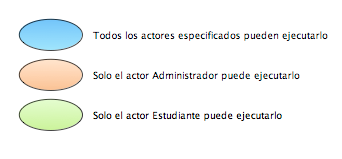
\includegraphics[width=0.8\textwidth]{images/CasosDeUso4}
		\caption{Diagrama de Casos de Uso del sistema.}
	\end{figure}
	
	\begin{figure}[htbp!]
		\centering
			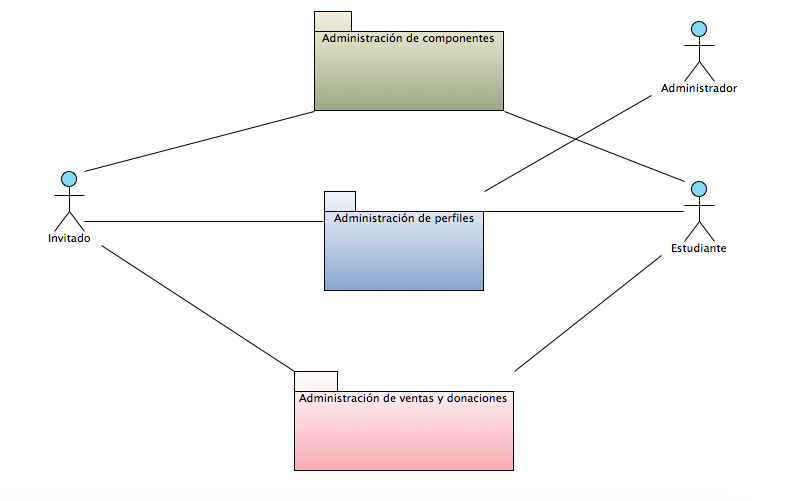
\includegraphics[width=1\textwidth]{images/CasosDeUso5}
		\caption{Diagrama de Casos de Uso del sistema.}
	\end{figure}
	
\cfinput{cu/cu12}
\cfinput{cu/cu13}
%\cfinput{cu1/cu}
%\cfinput{cu2/cu}
%\cfinput{cu3/cu}
%\cfinput{cu4/cu}
%\cfinput{cu5/cu}

%%=========================================================
\chapter{Modelo de la Interacción}

%\cfinput{Pantallas/navegacion}

\cfinput{Pantallas/IU5}
%\cfinput{Pantallas/IU1}
%\cfinput{Pantallas/IU2}
%\cfinput{Pantallas/IU3}
%\cfinput{Pantallas/IU4}
%\cfinput{Pantallas/IU5}
%\cfinput{Pantallas/IU6}
%\cfinput{Pantallas/IU7}

	
\end{document}
